\section{Market description}
\begin{frame}
	\frametitle{Customers and market potential}
	\begin{itemize}
		\item TSOs
			\begin{itemize}
				\item Approximately one per country
			\end{itemize}	
			\item Hydro power plant owners
			\begin{itemize}
				\item Approximately 1300 hydro power plants in Norway.
				\item Norway is the sixth largest hydro power plant producer in the world
			\end{itemize}
	\end{itemize}
\end{frame}
\begin{frame}
		\frametitle{Competition}
		\begin{columns}
				\begin{column}{0.4\textwidth}
						\begin{itemize}
								\item DNV GL offer a product according to the industry proposal.
								\item It requires disconnection of the plant.
								\item It takes very long time.
						\end{itemize}
				\end{column}
				\begin{column}{0.6\textwidth}
						\begin{figure}
								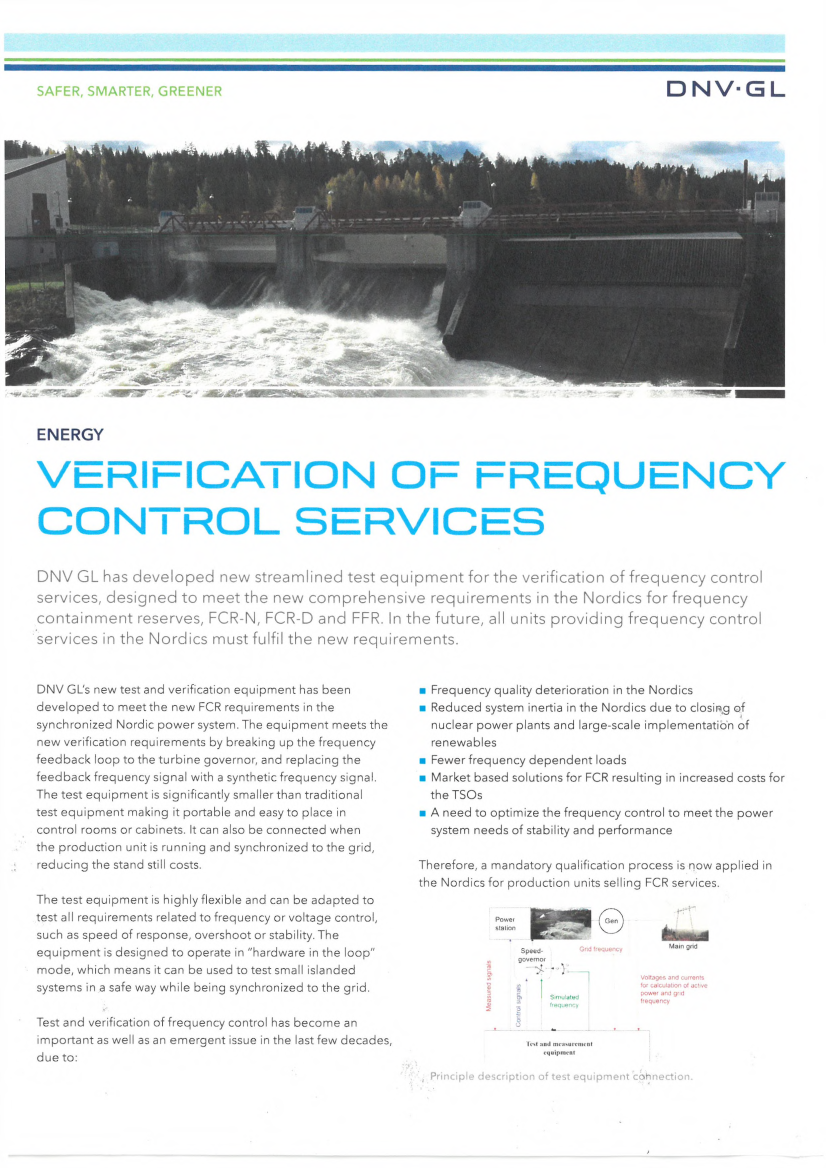
\includegraphics[width=\textwidth]{./pictures/DNV}
						\end{figure}
				\end{column}
		\end{columns}
\end{frame}
\begin{frame}
		\frametitle{IPR}
		\begin{itemize}
			\item Difficult to patent:
				\begin{itemize}
					\item Results have been published.
					\item Results rely on standard methods.
				\end{itemize}
			\item shared rights:
				\begin{itemize}
						\item NTNU
						\item Ampere Lab
						\item TTO renounced their rights
				\end{itemize}
\end{itemize}
\end{frame}
\begin{frame}
		\frametitle{Competitive advantage}
		\begin{itemize}
			\item We are the experts.
			\item We already have all the code and the know how.
			\item We have contacts in the industry.
			\item The industry are not likely to trust anyone.
			\item Our product is cheaper and more precise than the competition.
	\end{itemize}
	\end{frame}
